%%%%%%%% ICML 2018 EXAMPLE LATEX SUBMISSION FILE %%%%%%%%%%%%%%%%%

\documentclass{article}

% Recommended, but optional, packages for figures and better typesetting:
\usepackage{amsmath}
\usepackage{microtype}
\usepackage{graphicx}
\usepackage{subfigure}
\usepackage{booktabs} % for professional tables
\usepackage{amssymb}
\usepackage{multicol}
\usepackage{epstopdf}
% hyperref makes hyperlinks in the resulting PDF.
% If your build breaks (sometimes temporarily if a hyperlink spans a page)
% please comment out the following usepackage line and replace
% \usepackage{icml2018} with \usepackage[nohyperref]{icml2018} above.
\usepackage{hyperref}

% Attempt to make hyperref and algorithmic work together better:
\newcommand{\theHalgorithm}{\arabic{algorithm}}

% Use the following line for the initial blind version submitted for review:
\usepackage[accepted]{example/icml2018}

% If accepted, instead use the following line for the camera-ready submission:
%\usepackage[accepted]{icml2018}

% The \icmltitle you define below is probably too long as a header.
% Therefore, a short form for the running title is supplied here:
\icmltitlerunning{??}

\begin{document}

\twocolumn[
\icmltitle{??}

% It is OKAY to include author information, even for blind
% submissions: the style file will automatically remove it for you
% unless you've provided the [accepted] option to the icml2018
% package.

% List of affiliations: The first argument should be a (short)
% identifier you will use later to specify author affiliations
% Academic affiliations should list Department, University, City, Region, Country
% Industry affiliations should list Company, City, Region, Country

% You can specify symbols, otherwise they are numbered in order.
% Ideally, you should not use this facility. Affiliations will be numbered
% in order of appearance and this is the preferred way.
\icmlsetsymbol{equal}{*}

\begin{icmlauthorlist}
\icmlauthor{Meng Wang}{bmi}
\icmlauthor{Andrew J. Gentles}{bds}
\end{icmlauthorlist}

\icmlaffiliation{bmi}{Biomedical Informatics Training Program, Stanford University, CA, USA}
\icmlaffiliation{bds}{Department of Biomedical Data Sciences, Stanford University, CA, USA}
\icmlcorrespondingauthor{Andrew J. Gentles}{andrewg@stanford.edu}

% You may provide any keywords that you
% find helpful for describing your paper; these are used to populate
% the "keywords" metadata in the PDF but will not be shown in the document
\icmlkeywords{Machine Learning, ICML}

\vskip 0.3in
]

% this must go after the closing bracket ] following \twocolumn[ ...

% This command actually creates the footnote in the first column
% listing the affiliations and the copyright notice.
% The command takes one argument, which is text to display at the start of the footnote.
% The \icmlEqualContribution command is standard text for equal contribution.
% Remove it (just {}) if you do not need this facility.

\printAffiliationsAndNotice{}  % leave blank if no need to mention equal contribution
%\printAffiliationsAndNotice{\icmlEqualContribution} % otherwise use the standard text.

\begin{abstract} 

\end{abstract}

\section{Introduction}



\section{Methods}

%\begin{figure}[h]
%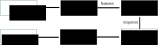
\includegraphics[width=0.5\textwidth]{../figs/flowChart}
%\caption{\textbf{Pipeline}}
%\end{figure}

\subsection{\citet{figueroa2010dna} DNA methylation and gene expression data}

DNA methylation and gene expression microarray data of 344 AML cases from \citet{figueroa2010dna} were downloaded from the GEO repository (GEO Accession number: GSE18700, GSE14468). Briefly, methylation data were obtained from custom design human promoter microarray for HELP assay, and gene expression data was obtained from Affymetrix Human Genome U133 Plus 2.0 Array. 

Preprocessed gene expression data were obtained from \citet{gentles2015prognostic}, which normalized the raw CEL files with Affymetrix MAS5 algorithm and $\log_2$ transformed. We queried the GO terms on molecular function and biological process based on the HUGO gene symbol of the probes and filtered for probes that contain keywords related to transcription and methylation, which serves as predictors of our model.

For methylation data analysis, we followed \citet{figueroa2010dna} and performed unsupervised hierarchical clustering of patients from methylation microarray using subset of the probes with standard deviation $> 1$ across all AML cases ($n = 3745$). Lingoes transformed 1 - Pearson correlation distance and Ward's minimum variance criterion were used. The patient clusters from the original study was reproduced. Next, we clustered the probes with similar methylation pattern using consensus clustering \citep{monti2003consensus}, which produces visual and quantitative stability evidence to a given number of clusters $k$ and cluster assignments. R package \texttt{ConsensusClusterPlus} \citep{wilkerson2010consensusclusterplus} provides an implementation of the method and were used to determine the optimal number of clusters. We used the following options: 80 \% probe subsampling, Ward's criterion with Lingoes transformation on 1 - Pearson correlation distance, 50 replicates for each $k$  and maximum $k = 10$.  We decides the number of optimal number of clusters based on the consensus matrix and area under CDF. The enrichment of biological processes represented by genes in each methylation cluster were examined using PANTHER overrepresentation test using Gene Ontology Biological process annotation data \citep{mi2013large} with $ FDR < 0.05$.

\subsection{Selection of significant gene expression probes}
Variational Bayesian spike regression (vBsr) \cite{logsdon2012novel} is a penalized Bayesian regression model that imposes sparsity constraint on the regression coefficients using a spike-and-slab prior and utilized mean-field approximation to achieve fast computation. In addition, the algorithm was ran multiple times with random initialization to identify multiple local maxima of lower bound and provides the option of Bayesian Model Averaging (BMA) over the identified models to produce an estimate to reduce the model uncertainty. vBsr also defines a test statistic $z_{vb}$ associated with each penalized coefficients that allow control over the family-wise error rate by tuning the penalty parameter $l_0$ such that $z_{vb}$ statistics are approximately $\mathcal{N}(0, 1)$ under the null hypothesis. We used vBsr to select the subset of gene expression probes that significantly associate with the observed pattern of variation of methylation level across patients. We ran 100 random starts for each model and used BMA option. We tuned the penalty parameter $l_0$ such that a feature will have a posterior probability of 0.95 if it passes a Bonferroni correction in the multivariate model to control the Type I error rate. Gene expression probes that were significant for $z_{vb}$ at $\widehat{FDR} = 0.1$ were selected. 

\begin{figure*}[htb!]
\centering
\includegraphics[width=\textwidth]{Figures/clustering}
\caption{\textbf{Consensus clustering of methylation probes for \citet{figueroa2010dna}} (a) consensus matrix for k = $6, 7, 8$. $k = 7$ shows high intra-cluster consensus and low intercluster consensus. (b) cumulative distribution function of consensus matrix at each $k = 1, \dots, 10$. $k = 7$ approaches the maximum consensus distribution (c) Area under CDF of consensus matrix for $k = 1, \dots, 10$. $k = 7$ is the largest $k$ with a appreciable increase in consensus (d) Hierarchical clustering of cases and probes. Each row represents a probe and each column represents a patients. Methylation intensity level were row and column normalized. The16 clusters of AML cases from \citet{figueroa2010dna} were reproduced. Probes were clustered using Ward's method with Pearson correlation distance transformed to Euclidean space and $k=7$ were chosen as the cutoff from CC.}
\label{CC}
\end{figure*}

\subsection{TCGA LAML RNA-seq and DNA methylation data}
TCGA Level 3 mRNAseq and DNA methylation data was downloaded from Broad TCGA GDAC site for LAML. mRNAseq probes with missing values were imputed by KNN using R packages \texttt{impute} \citep{hastie2001impute}. We queried the GO terms on molecular function and biological process based on the HUGO symbol of the probes and filtered for probes that contain keywords related to transcription and methylation as predictors for our model.   

Methylation array data was obtained from Illumina Infinium HumanMethylation450 BeadChip. Probes that are on chromosome X and Y were removed. Probes with UCSC RefGene group annotation as TSS 1500 and located within UCSC CpG island annotation were selected. The correlation between the Beta value of filtered methylation probes and RSEM level of the corresponding genes in mRNAseq data were computed and significant methylation probes was filtered with FDR adjusted p-value (FDR $< 0.1$) of 0.05. The resulting probes were clustered using hierarchical clustering with euclidean distance using Ward's method. 20 clusters were set as the cutoff for assigning cluster membership. The average methylation level within the cluster of each patient was computed as the response vector. 


\section{Results}

\subsection{Significant associated gene expression probes in \citet{figueroa2010dna}}

Figure \ref{CC} shows the results of consensus clustering on probes and significantly enriched biological processes in each cluster is shown below in Table \ref{enriched}. 

\begin{table*}[ht!]
\centering
\begin{tabular}{lllllllll}
  \toprule
Enriched biological process & ref & overlap & expected & fold enrich & raw P & FDR \\ 
  \midrule
  cluster 1 (size 326) \\
  \midrule
  cell communication & 5693 &  97 & 63.04 & 1.54 & 1.8e-6 & 2.4e-3 \\ 
  signaling & 5578 &  96 & 61.77 & 1.55 & 1.5e-6 & 2.3e-3 \\ 
   \midrule
   cluster 3 (size 671) \\
   \midrule
     cellular process & 15478 & 436 & 379.56 & 1.15 & 6.1e-9 & 9.5e-5 \\ 
\midrule
  cluster 5 (size 816)\\
  \midrule
  developmental process  & 5654 & 310 & 199.38 & 1.55 & 9.2e-18 & 1.4e-13 \\ 
  anatomical structure development & 5299 & 293 & 186.86 & 1.57 & 5.6e-17 & 4.4e-13 \\ 
  multicellular organism development & 4918 & 275 & 173.42 & 1.59 & 2.7e-16 & 1.1e-12 \\ 
  system development & 4309 & 244 & 151.95 & 1.61 & 1.0e-14 & 2.6e-11 \\ 
     \midrule
   cluster 6 (size 656)\\
  \midrule
  developmental process & 5654 & 199 & 147.52 & 1.35 & 2.2e-6 & 5.7e-3 \\ 
  cellular component organization or biogenesis & 5773 & 196 & 150.62 & 1.30 & 3.1e-5 & 2.7e-2 \\ 
  cellular component organization & 5584 & 192 & 145.69 & 1.32 & 2.0e-5 & 2.1e-2 \\ 
  anatomical structure development & 5299 & 190 & 138.25 & 1.37 & 1.3e-6 & 5.2e-3 \\ 
  multicellular organism development & 4918 & 184 & 128.31 & 1.43 & 1.1e-7 & 1.6e-3 \\ 
     \midrule
     cluster 7 (size 461) \\
     \midrule
     negative regulation of biological process & 5129 & 132 & 89.21 & 1.48 & 8.2e-07 & 1.3e-2 \\ 
	\bottomrule
\end{tabular}
\caption{\textbf{Enriched biological processes in \citet{figueroa2010dna} methylation probes cluster} }
\label{enriched}
\end{table*}



\section{Discussion}

\bibliography{main}
\bibliographystyle{example/icml2018}



\end{document}
